% ---------------------------------------------------------------------------
% Stage 1 presentation - Industrial Anomaly Detection on AutoVI
% AI for Trustworthy Decision Making
%
% Compile (from this folder):   pdflatex stage1_presentation.tex   (run twice)
% or upload the whole presentation/ folder to Overleaf.
%
% Where the numbers come from
%   Dataset, split, heterogeneity ..... notebooks/stage_01/data_lead.ipynb
%   PaDiM on the labelled split ....... notebooks/stage_01/baseline_model_with_markdowns.ipynb
%   Centralised vs federated .......... results/stage_01/*.json
%                                       (written by experiments/padim_experiment.py,
%                                        experiments/centralised.py, experiments/federated.py)
% Figures in figures/ are saved outputs of the notebooks and of padim_experiment.py.
% ---------------------------------------------------------------------------
\documentclass[aspectratio=169,10pt]{beamer}

\usepackage[utf8]{inputenc}
\usepackage[T1]{fontenc}
\usepackage{booktabs}
\usepackage{amsmath}
\usepackage{graphicx}
\usepackage{tikz}
\usetikzlibrary{positioning,arrows.meta}

% --- EDIT HERE: team, course, date ------------------------------------------
\newcommand{\teamauthors}{Bianca-Nicola Dragomir, Alexandra \textit{[surname]}, \textit{[third member]}}
\newcommand{\teamshort}{Dragomir, \textit{[surname]}, \textit{[third member]}}
\newcommand{\coursename}{AI for Trustworthy Decision Making}
\newcommand{\talkdate}{\today}
% -----------------------------------------------------------------------------

% --- Look: dark header with section dots, dark block titles, red highlights --
\usetheme{Frankfurt}
\definecolor{upbdark}{RGB}{35,31,32}
\definecolor{upbred}{RGB}{190,0,0}
\usecolortheme[named=upbdark]{structure}
\setbeamercolor{section in head/foot}{bg=upbdark,fg=white}
\setbeamercolor{frametitle}{bg=upbdark,fg=white}
\setbeamercolor{title}{bg=upbdark,fg=white}
\setbeamercolor{block title}{bg=upbdark,fg=white}
\setbeamercolor{block body}{bg=black!10,fg=black}
\setbeamercolor{block title alerted}{bg=upbred,fg=white}
\setbeamercolor{block body alerted}{bg=upbred!10,fg=black}
\setbeamercolor{alerted text}{fg=upbred!85!black}
\setbeamercolor{author in head/foot}{bg=upbdark,fg=white}
\setbeamercolor{title in head/foot}{bg=upbdark,fg=white}
\setbeamercolor{date in head/foot}{bg=upbdark,fg=white}
\setbeamertemplate{navigation symbols}{}
\setbeamertemplate{itemize items}[circle]
\setbeamertemplate{footline}{%
  \leavevmode%
  \hbox{%
  \begin{beamercolorbox}[wd=.42\paperwidth,ht=2.25ex,dp=1ex,left,leftskip=1ex]{author in head/foot}%
    \usebeamerfont{author in head/foot}\insertshortauthor
  \end{beamercolorbox}%
  \begin{beamercolorbox}[wd=.33\paperwidth,ht=2.25ex,dp=1ex,center]{title in head/foot}%
    \usebeamerfont{title in head/foot}\insertshorttitle
  \end{beamercolorbox}%
  \begin{beamercolorbox}[wd=.25\paperwidth,ht=2.25ex,dp=1ex,right,rightskip=1ex]{date in head/foot}%
    \usebeamerfont{date in head/foot}\insertshortdate\hspace*{2em}\insertframenumber{} / \inserttotalframenumber
  \end{beamercolorbox}}%
  \vskip0pt%
}

% Logos are optional: put upb.png, acs.png, ... in presentation/logos/ and they
% appear on the title and closing slides. Without the files nothing is drawn.
\newcommand{\optlogo}[1]{\IfFileExists{logos/#1}{\includegraphics[height=1.5cm]{logos/#1}\hspace{0.4cm}}{}}
\newcommand{\logorow}{\optlogo{upb.png}\optlogo{acs.png}\optlogo{logo3.png}\optlogo{logo4.png}}

\tikzset{
  box/.style={draw, rounded corners=2pt, fill=black!8, align=center,
              inner sep=4pt, font=\small, minimum height=0.9cm},
  hot/.style={box, fill=upbred!12, draw=upbred!80!black},
  arr/.style={-{Stealth[length=2mm]}, thick}
}

\title[Industrial Anomaly Detection on AutoVI]{Industrial Anomaly Detection on AutoVI}
\subtitle{Stage 1: centralised baseline and a minimal federated setup}
\author[\teamshort]{\teamauthors}
\institute{POLITEHNICA University of Bucharest\\
Faculty of Automatic Control and Computers\\
\coursename}
\date{\talkdate}

\begin{document}

% ===========================================================================
\begin{frame}[plain]
  \centering
  \logorow\par\vspace{0.3cm}
  \titlepage
\end{frame}

\begin{frame}{Outline}
  \tableofcontents
\end{frame}

% ===========================================================================
\section{Problem}

\begin{frame}{Problem}
  \begin{block}{Task}
    Decide from one photo whether a car part on the assembly line is
    \alert{correctly mounted} or \alert{defective}, and show where the defect is.
  \end{block}
  \begin{columns}[T]
    \begin{column}{0.48\textwidth}
      \begin{block}{Why unsupervised}
        \begin{itemize}
          \item Good parts are common, defects are rare.
          \item New defect types appear over time.
          \item The model learns only from \textbf{normal} images and flags
                what looks different.
        \end{itemize}
      \end{block}
    \end{column}
    \begin{column}{0.48\textwidth}
      \begin{block}{Why federated}
        \begin{itemize}
          \item Each inspection station keeps its own images.
          \item Stations differ: other parts, other lighting.
          \item Goal: one shared model, no images leaving a station.
        \end{itemize}
      \end{block}
    \end{column}
  \end{columns}
\end{frame}

\begin{frame}{Research questions}
  \begin{enumerate}
    \item How well does a simple unsupervised model (PaDiM) detect defects on
          real factory images?
    \item Does a model trained on \textbf{all} stations help or hurt each single
          station, compared with a model trained on that station alone?
    \item Can the same model be built \textbf{federated}, without pooling the
          images, and what is the cost in accuracy?
    \item How different are the stations from each other, measured in numbers?
  \end{enumerate}
  \vspace{0.3cm}
  \begin{alertblock}{Scope of Stage 1}
    Baseline, minimal federated setup, first results.
    Trust mechanisms (robustness, privacy, fairness, explanations) are Stage 2.
  \end{alertblock}
\end{frame}

% ===========================================================================
\section{Dataset}

\begin{frame}{AutoVI dataset (Renault Group)}
  \begin{columns}[T]
    \begin{column}{0.5\textwidth}
      \begin{itemize}
        \item Photos from real automotive assembly lines.
        \item We use the three categories delivered at $400\times400$ px.
        \item AutoVI's own split: training folder has \textbf{normal images only};
              all defects are in the test folder.
        \item Licence CC BY-NC-SA 4.0: images are not stored in our repository.
      \end{itemize}
    \end{column}
    \begin{column}{0.5\textwidth}
      \centering
      \small
      \begin{tabular}{lrrrr}
        \toprule
        Category & Normal & Defect & Total & Defect \% \\
        \midrule
        engine\_wiring & 570 & 322 & 892 & 36.1 \\
        pipe\_clip     & 390 & 142 & 532 & 26.7 \\
        pipe\_staple   & 379 & 117 & 496 & 23.6 \\
        \midrule
        All            & 1339 & 581 & 1920 & 30.3 \\
        \bottomrule
      \end{tabular}
      \par\vspace{0.2cm}
      {\footnotesize 8 defect types. \texttt{fastening} alone is 277 of the 581 defects.}
    \end{column}
  \end{columns}
\end{frame}

\begin{frame}{What the images look like}
  \centering
  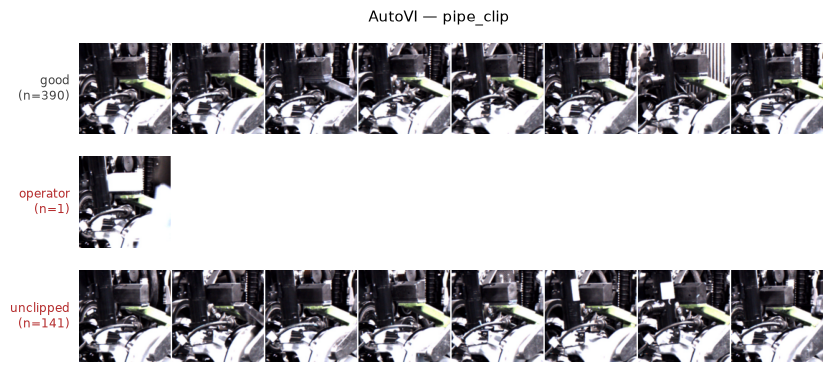
\includegraphics[height=0.72\textheight]{figures/data_examples_pipe_clip.png}
  \par{\footnotesize Category \texttt{pipe\_clip}: normal images (top) and its two defect types.
  AutoVI \copyright{} Renault Group, CC BY-NC-SA 4.0.}
\end{frame}

\begin{frame}{Data checks before training}
  \begin{columns}[T]
    \begin{column}{0.5\textwidth}
      \begin{block}{Exact duplicates}
        \begin{itemize}
          \item 73 images are byte-identical copies of another image
                (60 pairs in engine\_wiring, 13 in pipe\_clip).
          \item Removed: \textbf{1920 $\rightarrow$ 1847} images.
          \item No duplicate crosses two categories.
        \end{itemize}
      \end{block}
      \begin{block}{Format}
        \begin{itemize}
          \item All images $400\times400$.
          \item engine\_wiring is RGB, the other two are RGBA:
                everything is converted to RGB.
        \end{itemize}
      \end{block}
    \end{column}
    \begin{column}{0.5\textwidth}
      \begin{block}{Near-duplicates}
        \begin{itemize}
          \item 566 images (29.5\%) have a look-alike under an $8\times8$
                average hash.
          \item Expected: the camera and the part position are fixed.
        \end{itemize}
      \end{block}
      \begin{alertblock}{Leak check on the split}
        Train/validation $\cap$ test = 0 images.\\
        Any two clients share 0 images.\\
        Clients $\cup$ test cover all 1847 images.
      \end{alertblock}
    \end{column}
  \end{columns}
\end{frame}

% ===========================================================================
\section{Federated split}

\begin{frame}{One client per production part}
  \centering
  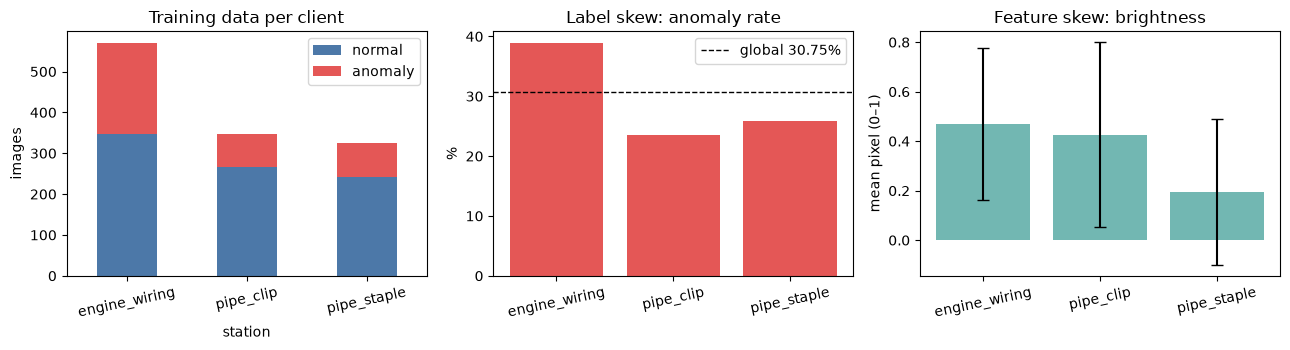
\includegraphics[width=0.78\textwidth]{figures/data_clients_skew.png}
  \par\vspace{0.1cm}
  \small
  \begin{tabular}{llrrrr}
    \toprule
    Client & Station & Train & Val & Defect \% & Mean brightness \\
    \midrule
    0 & engine\_wiring & 570 & 101 & 38.9 & 0.471 \\
    1 & pipe\_clip     & 348 & 62  & 23.6 & 0.426 \\
    2 & pipe\_staple   & 326 & 58  & 25.8 & 0.195 \\
    \midrule
    \multicolumn{2}{l}{Shared test set} & 382 & -- & 30.9 & 0.378 \\
    \bottomrule
  \end{tabular}
  \par{\footnotesize Labelled split (setup A in the results): 20\% test, seed 42.}
\end{frame}

\begin{frame}{How different are the clients?}
  \begin{columns}[T]
    \begin{column}{0.47\textwidth}
      \begin{block}{Three kinds of difference}
        \begin{itemize}
          \item \textbf{Size}: 570 / 348 / 326 images. Client 0 has about 46\% of the
                weight in a sample-weighted average.
          \item \textbf{Label}: defect rate 38.9\% / 23.6\% / 25.8\%.
          \item \textbf{Appearance}: pipe\_staple is less than half as bright.
                A linear model on 4 pixel statistics names the station
                correctly for \alert{97.3\%} of images.
        \end{itemize}
      \end{block}
    \end{column}
    \begin{column}{0.5\textwidth}
      \centering
      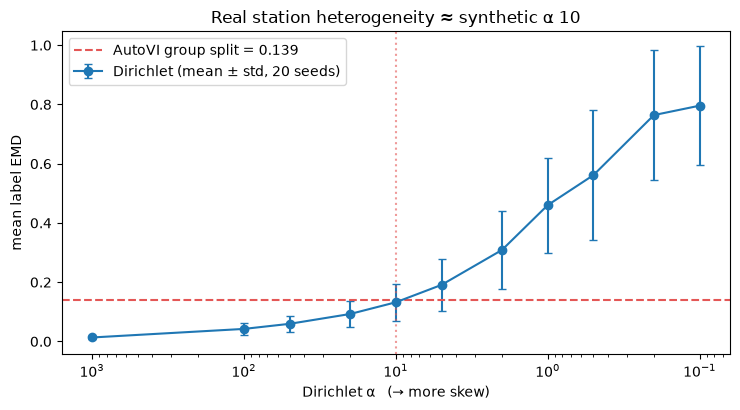
\includegraphics[width=\textwidth]{figures/data_dirichlet_scale.png}
      \par{\footnotesize Label difference of the real split (mean EMD 0.139) on the
      scale of synthetic Dirichlet splits: about $\alpha = 10$, a mild skew.}
    \end{column}
  \end{columns}
\end{frame}

\begin{frame}{Real split and stress-test splits}
  \centering
  \footnotesize
  \setlength{\tabcolsep}{4pt}
  \begin{tabular}{llrrrll}
    \toprule
    Strategy & Setting & Mean EMD & Mean JSD & Size Gini & Client sizes & Defect \% per client \\
    \midrule
    IID          & --           & 0.028 & 0.000 & 0.000 & 489 / 488 / 488  & 29.7 / 32.8 / 29.7 \\
    Dirichlet    & $\alpha=1.0$ & 0.387 & 0.045 & 0.229 & 375 / 293 / 797  & 34.7 / 68.9 / 14.8 \\
    Dirichlet    & $\alpha=0.1$ & 0.554 & 0.078 & 0.388 & 591 / 863 / 11   & 67.3 / 5.9 / 9.1 \\
    Pathological & 1 class      & 1.129 & 0.382 & 0.359 & 225 / 1015 / 225 & 100 / 0 / 100 \\
    \textbf{Group (real)} & \textbf{by station} & \textbf{0.139} & \textbf{0.004} & \textbf{0.131}
                 & \textbf{671 / 410 / 384} & \textbf{38.5 / 24.1 / 24.2} \\
    \bottomrule
  \end{tabular}
  \par\vspace{0.3cm}
  \begin{columns}[T]
    \begin{column}{0.48\textwidth}
      \begin{block}{Reading the table}
        EMD and JSD: difference between a client's label mix and the global one
        (0 = same). Gini: inequality of client sizes (0 = equal).
      \end{block}
    \end{column}
    \begin{column}{0.48\textwidth}
      \begin{alertblock}{Takeaway}
        The real stations differ mildly in labels and size, and strongly in
        appearance. The synthetic splits are kept as stress tests for Stage 2.
      \end{alertblock}
    \end{column}
  \end{columns}
\end{frame}

% ===========================================================================
\section{Model}

\begin{frame}{Baseline model: PaDiM}
  \centering
  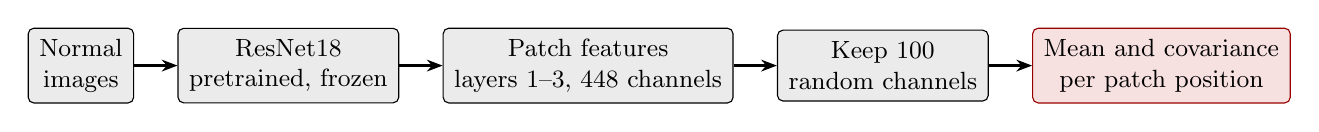
\begin{tikzpicture}[node distance=0.55cm]
    \node[box] (img) {Normal\\images};
    \node[box, right=of img] (cnn) {ResNet18\\pretrained, frozen};
    \node[box, right=of cnn] (emb) {Patch features\\layers 1--3, 448 channels};
    \node[box, right=of emb] (sub) {Keep 100\\random channels};
    \node[hot, right=of sub] (gau) {Mean and covariance\\per patch position};
    \draw[arr] (img) -- (cnn);
    \draw[arr] (cnn) -- (emb);
    \draw[arr] (emb) -- (sub);
    \draw[arr] (sub) -- (gau);
  \end{tikzpicture}
  \par\vspace{0.4cm}
  \begin{columns}[T]
    \begin{column}{0.48\textwidth}
      \begin{block}{Training}
        \begin{itemize}
          \item No gradient descent, no epochs.
          \item One pass over the normal images to compute the statistics.
          \item The only random choice is the channel subset (the seed).
        \end{itemize}
      \end{block}
    \end{column}
    \begin{column}{0.48\textwidth}
      \begin{block}{Scoring a new image}
        \begin{itemize}
          \item Mahalanobis distance of each patch to the statistics at its position
                gives an \textbf{anomaly map}.
          \item Image score = maximum of the smoothed map.
          \item Threshold = 95th percentile of the scores of normal validation images.
        \end{itemize}
      \end{block}
    \end{column}
  \end{columns}
\end{frame}

\begin{frame}{Federated setup}
  \centering
  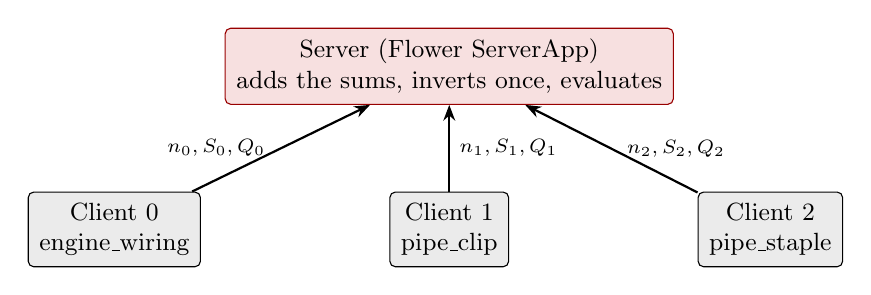
\begin{tikzpicture}[node distance=0.5cm and 1.1cm]
    \node[hot] (srv) {Server (Flower ServerApp)\\adds the sums, inverts once, evaluates};
    \node[box, below left=1.1cm and 0.3cm of srv] (c0) {Client 0\\engine\_wiring};
    \node[box, below=1.1cm of srv] (c1) {Client 1\\pipe\_clip};
    \node[box, below right=1.1cm and 0.3cm of srv] (c2) {Client 2\\pipe\_staple};
    \draw[arr] (c0) -- node[left, font=\scriptsize, xshift=-2pt] {$n_0, S_0, Q_0$} (srv);
    \draw[arr] (c1) -- node[right, font=\scriptsize] {$n_1, S_1, Q_1$} (srv);
    \draw[arr] (c2) -- node[right, font=\scriptsize, xshift=2pt] {$n_2, S_2, Q_2$} (srv);
  \end{tikzpicture}
  \par\vspace{0.2cm}
  \begin{columns}[T]
    \begin{column}{0.5\textwidth}
      \begin{block}{What a client sends}
        Per patch position, over its own normal images:
        \[ S_k=\sum_i x_i, \qquad Q_k=\sum_i x_i x_i^{\top}, \qquad n_k \]
        No image and no per-image value leaves the client.
      \end{block}
    \end{column}
    \begin{column}{0.47\textwidth}
      \begin{block}{What the server does}
        \[ \mu=\frac{\sum_k S_k}{\sum_k n_k}, \qquad
           \Sigma=\frac{n}{n-1}\Bigl(\frac{\sum_k Q_k}{n}-\mu\mu^{\top}\Bigr) \]
        A sample-weighted average, as in FedAvg, but \alert{one round} and
        \alert{exact}.
      \end{block}
    \end{column}
  \end{columns}
\end{frame}

\begin{frame}{Metrics}
  \begin{columns}[T]
    \begin{column}{0.48\textwidth}
      \begin{block}{Without a threshold}
        \begin{itemize}
          \item \textbf{AUROC}: how well scores rank defects above normal parts.
                0.5 = random, 1.0 = perfect.
          \item \textbf{AP}: area under the precision--recall curve.
        \end{itemize}
      \end{block}
      \begin{block}{Why not plain accuracy}
        About 70\% of images are normal, so a model that always answers
        ``normal'' already reaches about 70\% accuracy.
      \end{block}
    \end{column}
    \begin{column}{0.48\textwidth}
      \begin{block}{With the threshold}
        \begin{itemize}
          \item \textbf{TPR}: share of defects that are caught.
          \item \textbf{TNR}: share of good parts that are accepted.
          \item \textbf{Balanced accuracy} = (TPR + TNR) / 2.
          \item \textbf{Macro-F1}.
        \end{itemize}
      \end{block}
      \begin{alertblock}{Reporting}
        Mean $\pm$ standard deviation over seeds 1, 2, 3.
      \end{alertblock}
    \end{column}
  \end{columns}
\end{frame}

% ===========================================================================
\section{Results}

\begin{frame}{Two evaluation setups}
  \centering
  \small
  \begin{tabular}{p{2.6cm}p{5.3cm}p{5.3cm}}
    \toprule
     & \textbf{A. Labelled split} & \textbf{B. Official AutoVI split} \\
    \midrule
    Built by & our re-split by category, 20\% test, seed 42 & AutoVI's own train and test folders \\
    Clients & 3 (one per part) & 3 (one per part) \\
    Train, normal images & 348 / 266 / 242 (856) & 242 / 166 / 162 (570) \\
    Defects in train/val & yes (PaDiM ignores those in train) & none \\
    Test set & 382 images: 264 normal, 118 defects & 1176 images: 608 normal, 568 defects \\
    Image size & $128\times128$ & $128\times128$ \\
    Used for & PaDiM notebook, supervised CNN & PaDiM centralised vs.\ federated \\
    \bottomrule
  \end{tabular}
  \par\vspace{0.3cm}
  \begin{alertblock}{Why two}
    PaDiM follows the dataset's own protocol (B), so it can be set next to the
    published scores. The supervised CNN needs defects in training, which only the
    labelled re-split (A) provides. Numbers from A and B are not comparable with each other.
  \end{alertblock}
\end{frame}

\begin{frame}{PaDiM on the labelled split (setup A, baseline notebook)}
  \begin{columns}[T]
    \begin{column}{0.4\textwidth}
      \small
      \begin{tabular}{lcc}
        \toprule
        Metric & Validation & Test \\
        \midrule
        AUROC         & $0.703 \pm 0.016$ & $0.654 \pm 0.001$ \\
        AP            & $0.528 \pm 0.009$ & $0.473 \pm 0.013$ \\
        Balanced acc. & $0.607 \pm 0.012$ & $0.564 \pm 0.011$ \\
        Macro-F1      & $0.614 \pm 0.016$ & $0.546 \pm 0.019$ \\
        TPR           & $0.263 \pm 0.025$ & $0.175 \pm 0.030$ \\
        TNR           & $0.950 \pm 0.000$ & $0.952 \pm 0.008$ \\
        \bottomrule
      \end{tabular}
      \par\vspace{0.2cm}
      {\footnotesize One model fitted on the 856 normal training images of all
      clients. Mean $\pm$ std over seeds 1, 2, 3.}
    \end{column}
    \begin{column}{0.58\textwidth}
      \centering
      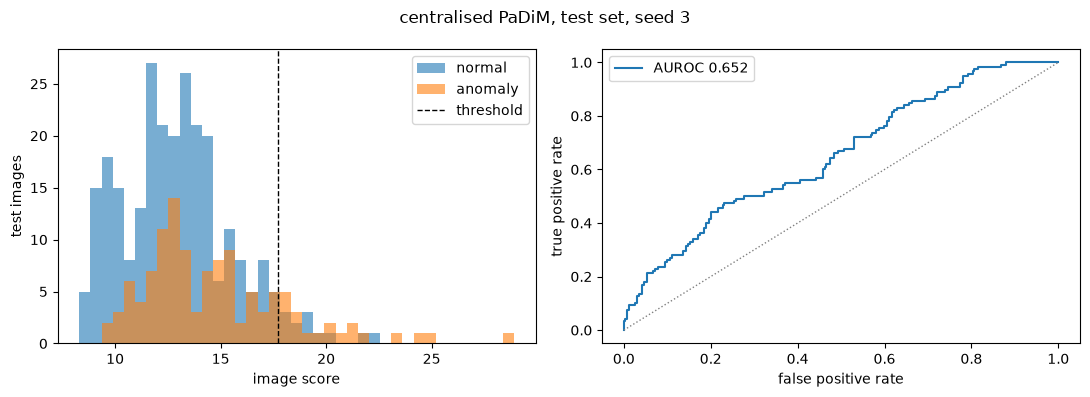
\includegraphics[width=\textwidth]{figures/base_scores_roc.png}
    \end{column}
  \end{columns}
  \vspace{0.1cm}
  \begin{alertblock}{Reading}
    The ranking is better than random, but with 95\% of good parts accepted only
    about 1 defect in 6 is caught: the two score distributions overlap.
  \end{alertblock}
\end{frame}

\begin{frame}{Pooled model vs.\ one model per client (setup A)}
  \centering
  \small
  \begin{tabular}{clrcccc}
    \toprule
           &         &            & \multicolumn{2}{c}{AUROC} & \multicolumn{2}{c}{Balanced accuracy} \\
    \cmidrule(lr){4-5}\cmidrule(lr){6-7}
    Client & Station & Val images & Pooled & Local & Pooled & Local \\
    \midrule
    0 & engine\_wiring & 101 & $0.743 \pm 0.025$ & $0.761 \pm 0.014$ & $0.650 \pm 0.015$ & $0.617 \pm 0.032$ \\
    1 & pipe\_clip     & 62  & $0.646 \pm 0.056$ & $0.730 \pm 0.043$ & $0.565 \pm 0.034$ & $0.535 \pm 0.045$ \\
    2 & pipe\_staple   & 58  & $0.618 \pm 0.083$ & $0.776 \pm 0.058$ & $0.502 \pm 0.030$ & $0.488 \pm 0.032$ \\
    \bottomrule
  \end{tabular}
  \par\vspace{0.25cm}
  \begin{columns}[T]
    \begin{column}{0.48\textwidth}
      \begin{block}{Observation}
        In AUROC, every station is served \textbf{better by its own model} than by
        the pooled one. The gap is small for engine\_wiring and large for
        pipe\_staple ($0.618$ vs.\ $0.776$).
      \end{block}
    \end{column}
    \begin{column}{0.48\textwidth}
      \begin{alertblock}{Likely reason}
        PaDiM keeps one mean and covariance per image position. Three different
        parts at the same position give a wide ``normal'' that hides small defects.
        The stations differ strongly in appearance (97.3\% separable).
      \end{alertblock}
    \end{column}
  \end{columns}
\end{frame}

\begin{frame}{Where the model looks: anomaly maps}
  \centering
  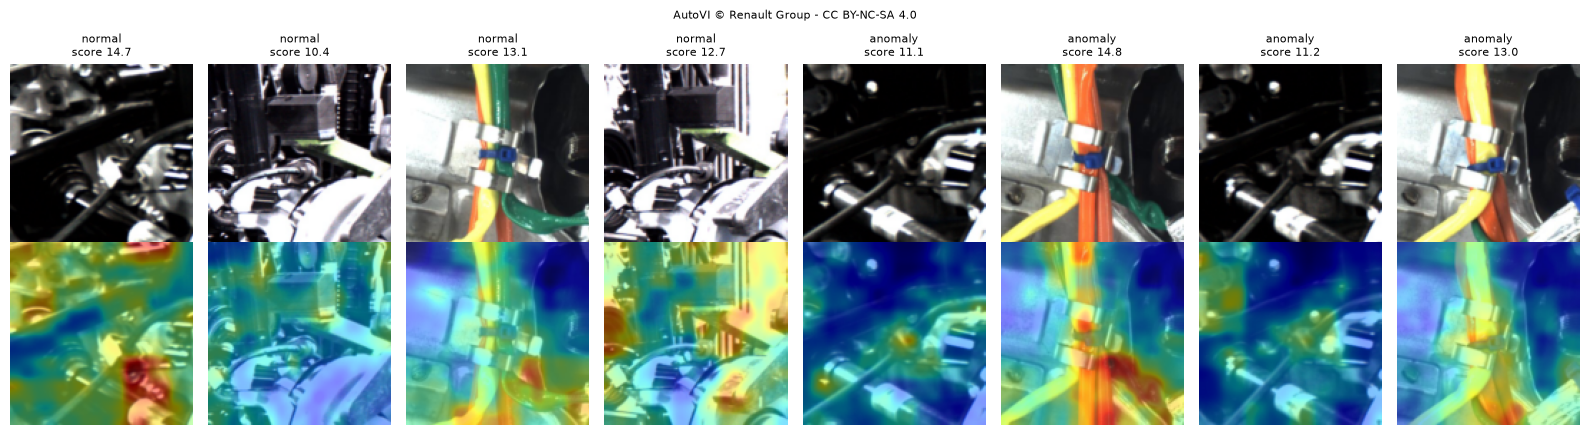
\includegraphics[width=0.98\textwidth]{figures/base_anomaly_maps.png}
  \par{\footnotesize Four normal and four defective test images with the pooled model's
  anomaly maps (red = far from the learned normal appearance). The map comes from
  the model itself. Some normal images also show red areas, in line with the
  modest scores: the maps are not yet a reliable explanation.}
\end{frame}

\begin{frame}{Federated vs.\ centralised: PaDiM (setup B)}
  \begin{columns}[T]
    \begin{column}{0.56\textwidth}
      \footnotesize
      \setlength{\tabcolsep}{4pt}
      \begin{tabular}{lccc}
        \toprule
        Training & AUROC & AP & Bal.\ acc. \\
        \midrule
        Centralised (pooled images)   & $0.624 \pm 0.017$ & $0.619 \pm 0.012$ & $0.564 \pm 0.009$ \\
        Federated, Flower, 1 round    & $0.624 \pm 0.017$ & $0.619 \pm 0.012$ & $0.564 \pm 0.009$ \\
        Federated, in-process         & $0.624 \pm 0.017$ & $0.619 \pm 0.012$ & $0.564 \pm 0.009$ \\
        \midrule
        Local models, mean of 3       & $0.648 \pm 0.026$ & $0.563 \pm 0.021$ & $0.538 \pm 0.005$ \\
        \bottomrule
      \end{tabular}
      \par\vspace{0.15cm}
      {\footnotesize Global test set, seeds 1, 2, 3. Per seed, the federated and
      centralised AUROC differ by at most $2\times10^{-6}$.}
      \par\vspace{0.2cm}
      \begin{tabular}{lccc}
        \toprule
        AUROC on own test slice & Pooled & Local & Paper \\
        \midrule
        engine\_wiring & $0.728$ & $0.726$ & $0.792$ \\
        pipe\_clip     & $0.510$ & $0.566$ & $0.626$ \\
        pipe\_staple   & $0.509$ & $0.651$ & $0.546$ \\
        \bottomrule
      \end{tabular}
      \par\vspace{0.1cm}
      {\footnotesize Paper: PaDiM per category in Carvalho et al.\ (2024), at a larger image size.}
    \end{column}
    \begin{column}{0.42\textwidth}
      \begin{block}{Result}
        The federated model \alert{is} the centralised model: no accuracy is lost
        by keeping the images at the stations.
      \end{block}
      \begin{alertblock}{But}
        The shared model is weak for pipe\_clip and pipe\_staple (AUROC near 0.5).
        Federation reproduces pooling exactly, including its weakness.
      \end{alertblock}
    \end{column}
  \end{columns}
\end{frame}

\begin{frame}{Federated vs.\ centralised: supervised CNN with FedAvg (setup A)}
  \begin{columns}[T]
    \begin{column}{0.6\textwidth}
      \footnotesize
      \setlength{\tabcolsep}{4pt}
      \begin{tabular}{lccc}
        \toprule
        Training & Accuracy & Bal.\ acc. & Macro-F1 \\
        \midrule
        Centralised, 10 epochs        & $0.913 \pm 0.012$ & $0.887 \pm 0.008$ & $0.896 \pm 0.013$ \\
        FedAvg, Flower, 10 rounds     & $0.869 \pm 0.009$ & $0.849 \pm 0.003$ & $0.847 \pm 0.008$ \\
        FedAvg, in-process, 10 rounds & $0.866 \pm 0.020$ & $0.854 \pm 0.009$ & $0.846 \pm 0.018$ \\
        \bottomrule
      \end{tabular}
      \par\vspace{0.15cm}
      {\footnotesize Test set of 382 images, seeds 1, 2, 3. Small CNN classifier, 1 local epoch per round,
      3 clients, sample-weighted averaging.}
      \par\vspace{0.25cm}
      \begin{tabular}{lcc}
        \toprule
        Worst client, validation bal.\ acc. & Centralised & FedAvg (Flower) \\
        \midrule
        & $0.854 \pm 0.009$ & $0.788 \pm 0.030$ \\
        \bottomrule
      \end{tabular}
    \end{column}
    \begin{column}{0.38\textwidth}
      \begin{block}{Result}
        FedAvg costs about \alert{3 to 4 points} of balanced accuracy against
        centralised training, and more for the worst-served client.
      \end{block}
      \begin{block}{Caveat}
        This model \textbf{sees defects in training}. It can only recognise the
        defect types it was shown, and its scores cannot be compared with PaDiM's.
      \end{block}
    \end{column}
  \end{columns}
\end{frame}

% ===========================================================================
\section{Next steps}

\begin{frame}{Limitations observed in Stage 1}
  \begin{itemize}
    \item \textbf{Unsupervised detection is modest.} Test AUROC 0.62 to 0.65; most
          defects are missed when 95\% of good parts are accepted.
    \item \textbf{Small images.} All runs use $128\times128$ inputs; the originals are
          $400\times400$ and some defects are small.
    \item \textbf{One shared model for three different parts.} Pooling, and therefore
          federation, is worse than a local model for two of the three stations.
    \item \textbf{Comparison with the paper is indirect.} The paper uses a larger
          image size; our local models reach 0.726 / 0.566 / 0.651 AUROC against
          0.792 / 0.626 / 0.546 published.
    \item \textbf{The supervised CNN is not a like-for-like alternative.} It needs
          labelled defects, which AutoVI's protocol does not provide for training.
    \item \textbf{Statistics are not private by default.} $S_k/n_k$ is the
          client's mean feature map.
    \item \textbf{Three of the six AutoVI categories} are used (those delivered at
          $400\times400$).
  \end{itemize}
\end{frame}

\begin{frame}{Stage 2: trust dimensions}
  \begin{columns}[T]
    \begin{column}{0.48\textwidth}
      \begin{block}{Robustness}
        A client that sends statistics computed on defective or shifted images:
        how much does the shared model degrade, and can the server notice?
      \end{block}
      \begin{block}{Fairness across stations}
        Report the worst-served station next to the average; test a shared
        backbone with per-station statistics or thresholds.
      \end{block}
    \end{column}
    \begin{column}{0.48\textwidth}
      \begin{block}{Privacy}
        Add calibrated noise to $S_k$ and $Q_k$ and measure the AUROC cost.
        The gradient-based differential privacy of the starter kit does not apply.
      \end{block}
      \begin{block}{Interpretability}
        Score the anomaly maps against AutoVI's defect masks, not only by eye.
      \end{block}
    \end{column}
  \end{columns}
  \vspace{0.2cm}
  \begin{alertblock}{Requirement}
    The team must cover at least two of these and compare
    centralised vs.\ federated vs.\ trust-enhanced versions.
  \end{alertblock}
\end{frame}

\begin{frame}{References}
  \footnotesize
  \begin{thebibliography}{9}
    \bibitem{autovi} P. Carvalho, M. Lafou, A. Durupt, A. Leblanc, Y. Grandvalet.
      Detecting visual anomalies in an industrial environment: Unsupervised methods
      put to the test on the AutoVI dataset. \emph{Computers in Industry} 163, 104151, 2024.
    \bibitem{padim} T. Defard, A. Setkov, A. Loesch, R. Audigier.
      PaDiM: a Patch Distribution Modeling Framework for Anomaly Detection and
      Localization. \emph{ICPR Workshops}, 2021.
    \bibitem{fedavg} H. B. McMahan, E. Moore, D. Ramage, S. Hampson, B. A. y Arcas.
      Communication-Efficient Learning of Deep Networks from Decentralized Data.
      \emph{AISTATS}, 2017.
    \bibitem{kairouz} P. Kairouz, H. B. McMahan, et al.
      Advances and Open Problems in Federated Learning.
      \emph{Foundations and Trends in Machine Learning} 14(1--2), 2021.
    \bibitem{hsu} T.-M. H. Hsu, H. Qi, M. Brown.
      Measuring the Effects of Non-Identical Data Distribution for Federated Visual
      Classification. arXiv:1909.06335, 2019.
    \bibitem{flower} D. J. Beutel, et al.
      Flower: A Friendly Federated Learning Framework. arXiv:2007.14390, 2020.
  \end{thebibliography}
\end{frame}

\begin{frame}[plain]
  \centering
  {\Huge Thank you for your attention!}
  \par\vspace{1cm}
  \logorow
\end{frame}

\end{document}
